\documentclass{article}
\usepackage[margin=.5in]{geometry}
\usepackage{tikz}
\begin{document}
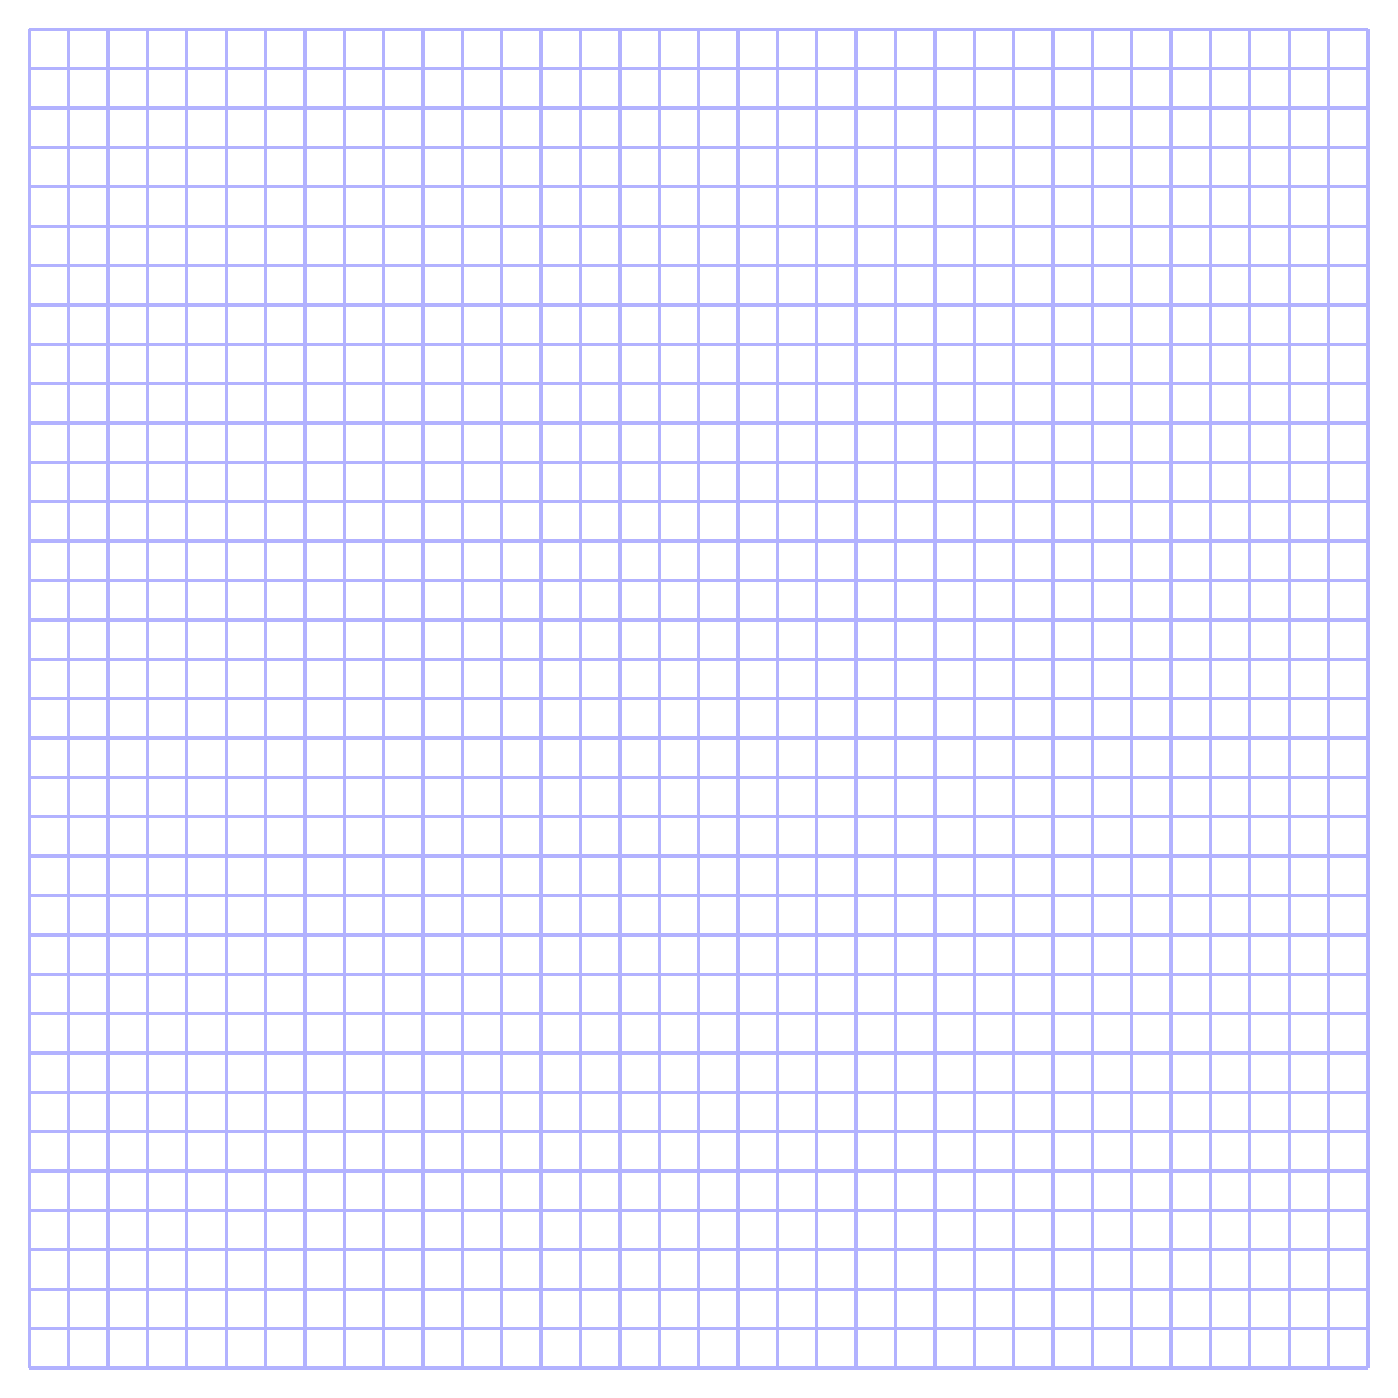
\begin{tikzpicture}
%\begin{axis}[width=\marginparwidth+25pt,tick label style={font=\scriptsize},minor x tick num=1, axis y line=middle,axis x line=middle,ymin=-3.1,ymax=8.1,xmin=-7.5,xmax=6.5,name=myplot]
%\addplot [thin,dashed] coordinates {(-7.5,5) (6.5,5)};
%\addplot [thick,white,smooth,domain=-7.5:6.5] {(5*(x-2)*(x+1))/(x^2+2*x+4)};
%
%\filldraw [{\colorone}] (axis cs:-5.75,7.2) circle (1pt);
%\filldraw [{\colorone}] (axis cs:-4., 7.5) circle (1pt);
%\filldraw [{\colorone}] (axis cs:-1.31, 1.63) circle (1pt);
%\filldraw [{\colorone}] (axis cs:-1,0) circle (1pt);
%\filldraw [{\colorone}] (axis cs:0., -2.5) circle (1pt);
%\filldraw [{\colorone}] (axis cs:1.064, -1.33) circle (1pt);
%\filldraw [{\colorone}] (axis cs:2,0) circle (1pt);
%\end{axis}
%
%\node [right] at (myplot.right of origin) {\scriptsize $x$};
%\node [above] at (myplot.above origin) {\scriptsize $y$};

\draw[draw=blue!30!white,very thick] (0,0) grid [step=.5] (17,17);

\end{tikzpicture}


\end{document}